\documentclass{ctexbook}
\usepackage[T1]{fontenc}
\PassOptionsToPackage{dvipsnames,svgnames}{xcolor}
\usepackage{graphicx,rotating,float,booktabs}
\usepackage[object=vectorian]{pgfornament}
\usetikzlibrary{shapes.geometric,calc}
\usepackage{tkzexample,tikzrput,pict2e,picture}
\usepackage{eso-pic,calc}
\setmainfont{Times New Roman}
\usepackage[centering,
           top=2.54cm,bottom=2.54cm,right=2cm,left=2cm,
           headsep=25pt,headheight=20pt]{geometry}
\usepackage{hyperref,tkzexample}
\usepackage{eso-pic}
\makeatletter
\AddToShipoutPicture{%
\begingroup
\setlength{\@tempdima}{2mm}%
\setlength{\@tempdimb}{\paperwidth-\@tempdima-2cm}%
\setlength{\@tempdimc}{\paperheight-\@tempdima}%
\put(\LenToUnit{\@tempdima},\LenToUnit{\@tempdimc}){%
 \pgfornament[anchor=north west,width=2cm,color=Maroon]{63}}
\put(\LenToUnit{\@tempdima},\LenToUnit{\@tempdima}){%
  \pgfornament[anchor=south west,width=2cm,symmetry=h,color=Maroon]{63}}
\put(\LenToUnit{\@tempdimb},\LenToUnit{\@tempdimc}){%
  \pgfornament[anchor=north east,width=2cm,symmetry=v,color=Maroon]{63}}
\put(\LenToUnit{\@tempdimb},\LenToUnit{\@tempdima}){%
  \pgfornament[anchor=south east,width=2cm,symmetry=c,color=Maroon]{63}}
\endgroup
}
\makeatother
\hypersetup{%
pdfauthor = {向禹},
pdftitle = {pgfornament},
pdfsubject = {pgfornament使用说明},
colorlinks=true,
linkcolor=red,
urlcolor=blue}
\definecolor{Maroon}{rgb}{0.5,0,0}


\begin{document}
\chapter*{pgfornament——一个给你花样装饰的宏包}
这次给大家介绍一个宏包——pgfornament,可以给文档添加非常漂亮的装饰效果,尤其是在封面制作,幻灯片演示方面应该有很好的应用。林莲枝老师在此包的基础上扩展编写了中文版本的pgfornament-han包,加入了很多中国的元素,也值得大家参考,但是这里的话我们只介绍pgfornament包的使用。

要使用此宏包,您只需要在导言区加入\verb|\usepackage{pgfornament}|或者\verb|\usepackage[object=vectorian]|\\
\texttt{{pgfornament}},此包会自动加载Ti$k$Z包。\verb|\pgfornament|命令画出一个指定的数字对应的矢量图,这个命令可以单独用,也可以放在一个\verb|picture|环境中,事实上此命令就是由当前位置的一个\verb|tikzpicture|环境所定义的。

\verb|\pgfornament|的完整命令如下
\begin{verbatim}
\pgfornament[<options>]{number}
\end{verbatim}

这里的数字参数范围是1-196,也就是本包中自定义的196个矢量图,大家可以查看pgfornament的源文档说明,命令行输入texdoc pgfornament即可,第17页开始列出了所有的矢量图。\\
\begin{minipage}{0.6\textwidth}
\begin{tkzexample}[code only,width=5cm,small]
  \usepackage{ornament}
  ...
  \pgfornament[width=2cm]{1}
\end{tkzexample}
您可以得到图\ref{fig:o1}
\end{minipage}
\begin{minipage}{0.4\textwidth}
\begin{figure}[H]
 \begin{center}
  \pgfornament[width=2cm,color=Maroon]{1}
\end{center}
  \caption{矢量图1}
  \label{fig:o1}
\end{figure}
\end{minipage}
\begin{minipage}{0.6\textwidth}
\begin{tkzexample}[code only,width=5cm,small]
  \usepackage{ornament}
  ...
  \pgfornament[width=2cm]{4}
\end{tkzexample}
您可以得到图\ref{fig:o2}
\end{minipage}
\begin{minipage}{0.4\textwidth}
\begin{figure}[H]
 \begin{center}
  \pgfornament[width=2cm,color=Maroon]{4}
\end{center}
  \caption{矢量图2}
  \label{fig:o2}
\end{figure}
\end{minipage}

此命令含有6个可选参数:\texttt{scale,width,height,color,opacity,ydelta,symmetry},其中最后一个几何变换参数\texttt{symmetry}有四种选择。

\begin{table}[h]\centering
{ \small   \begin{tabular}{lll}
      \toprule
参数 & 默认值  &  定义 \\
\midrule
\texttt{scale}          & 1          &图片的宽度和高度不变\\
\texttt{width}          & \{\}       & 设置宽度,宽高比不变  \\
\texttt{height}         & \{\}       & 设置高度,宽高比不变\\
\texttt{color}          & black      & 图片颜色 \\
\texttt{opacity}        & 1          & 图片透明度 \\
\texttt{ydelta}         & 0 pt       & 图片的垂直平移 \\
\texttt{symmetry=v}     & none       & 垂直轴对称\\
\texttt{symmetry=h}     & none       & 水平轴对称\\
\texttt{symmetry=c}     & none       & 中心对称\\
\texttt{symmetry=none}  & none       & 默认不作变换\\
\bottomrule
\end{tabular} }
\caption{pgfornament包的可选项}
  \label{tab:pgfornament-options}
\end{table}

\begin{enumerate}\setlength{\itemsep}{30pt}
\begin{minipage}[t]{0.6\textwidth}
\item \texttt{scale}选项
\begin{tkzexample}[code only,small]
  \pgfornament[scale=0.25]{77}
\end{tkzexample}
\end{minipage}
\begin{minipage}{0.4\textwidth}
  \pgfornament[scale=0.25,color=Maroon]{77}
\end{minipage}

\begin{minipage}[t]{0.6\textwidth}
\item \texttt{width}选项
\begin{tkzexample}[code only,small]
 \pgfornament[width=5cm]{77}
\end{tkzexample}
\end{minipage}
\begin{minipage}{0.4\textwidth}
  \pgfornament[width=5cm,color=Maroon]{77}
\end{minipage}

\begin{minipage}[t]{0.6\textwidth}
\item \texttt{height}选项
\begin{tkzexample}[code only,small]
\pgfornament[height=1cm]{77}
\end{tkzexample}
\end{minipage}
\begin{minipage}{0.4\textwidth}
  \pgfornament[height=1cm,color=Maroon]{77}
\end{minipage}

\begin{minipage}[t]{0.6\textwidth}
\item \texttt{color}选项
\begin{tkzexample}[code only,small]
\pgfornament[height=1cm,color=green!20!black]{77}
\end{tkzexample}
\end{minipage}
\begin{minipage}{0.4\textwidth}
\pgfornament[height=1cm,color=green!20!black]{77}
\end{minipage}

\begin{minipage}[t]{0.6\textwidth}
\item \texttt{opacity}选项
\begin{tkzexample}[code only,small]
\pgfornament[height=1cm,color=green!20!black,opacity=0.2]{77}
\end{tkzexample}
\end{minipage}
\begin{minipage}{0.4\textwidth}
\pgfornament[height=1cm,color=green!20!black,opacity=0.2]{77}
\end{minipage}

\begin{minipage}[t]{0.6\textwidth}
\item \texttt{symmetry=h}选项
\begin{tkzexample}[code only,small]
\pgfornament[height=1cm,symmetry=h]{77}
\end{tkzexample}
\end{minipage}
\begin{minipage}{0.4\textwidth}
\pgfornament[height=1cm,symmetry=h,color=Maroon]{77}
\end{minipage}

\begin{minipage}[t]{0.6\textwidth}
\item \texttt{symmetry=v}选项
\begin{tkzexample}[code only,small]
\pgfornament[height=1cm,symmetry=v]{77}
\end{tkzexample}
\end{minipage}
\begin{minipage}{0.4\textwidth}
\pgfornament[height=1cm,symmetry=v,color=Maroon]{77}
\end{minipage}

\begin{minipage}[t]{0.6\textwidth}
\item \texttt{symmetry=c}选项
\begin{tkzexample}[code only,small]
\pgfornament[height=1cm,symmetry=c]{77}
\end{tkzexample}
\end{minipage}
\begin{minipage}{0.4\textwidth}
 \pgfornament[height=1cm,symmetry=c,color=Maroon]{77}
\end{minipage}
\end{enumerate}

对称选项的例子
\begin{enumerate}
  \item 垂直轴对称
\tikzset{pgfornamentstyle/.style={draw=green!20!black,
           fill=orange,fill opacity=.5,thick}}%

  \begin{figure}[H]
	  \fbox{\pgfornament[width=5cm]{2}}%
	  \pgfornament[width=5cm,symmetry=v]{2}
	  \caption{Vertical symmetry}
  \end{figure}


 \item 水平轴对称
\tikzset{pgfornamentstyle/.style={draw=green!20!black,
           fill=orange,fill opacity=.5,thick}}%

  \begin{figure}[H]
 \fbox{\pgfornament[width=5cm]{2}}%
  \pgfornament[width=5cm,symmetry=h]{2}
	\caption{Horizontal symmetry}
  \end{figure}

 \item 原点中心对称
\tikzset{pgfornamentstyle/.style={draw=green!20!black,
           fill=orange,fill opacity=.5,thick}}%

  \fbox{\pgfornament[width=5cm]{2}}%

  \hspace*{5cm}
    \begin{figure}[H]
  \pgfornament[width=5cm,symmetry=c]{2}%
  	  \caption{Central symmetry}
  \end{figure}
\end{enumerate}

\texttt{ydelta}选项\\
\begin{minipage}{0.6\textwidth}
\begin{tkzexample}[code only,small]
  \pgfornament[color=MidnightBlue,width=2cm,ydelta=-10pt]{25}%
  \pgfornament[color=PineGreen,width=2cm]{25}%
  \pgfornament[color=Periwinkle,width=2cm,ydelta=+10pt]{25}%
\end{tkzexample}
\end{minipage}
\begin{minipage}{0.4\textwidth}%
  \pgfornament[color=MidnightBlue,width=2cm,ydelta=-10pt]{25}%
  \pgfornament[color=PineGreen,width=2cm]{25}%
  \pgfornament[color=Periwinkle,width=2cm,ydelta=+10pt]{25}%
\end{minipage}

除此之外,还可以借助\verb|eso-pic|包给文档的每一页的四个角落增加一个对称的装饰,正如本文档一样,导言区加入如下代码即可。

\begin{tkzexample}[code only,small]
\usepackage{eso-pic}
\makeatletter
\AddToShipoutPicture{%
\begingroup
\setlength{\@tempdima}{2mm}%
\setlength{\@tempdimb}{\paperwidth-\@tempdima-2cm}%
\setlength{\@tempdimc}{\paperheight-\@tempdima}%
\put(\LenToUnit{\@tempdima},\LenToUnit{\@tempdimc}){%
 \pgfornament[anchor=north west,width=2cm]{63}}
\put(\LenToUnit{\@tempdima},\LenToUnit{\@tempdima}){%
  \pgfornament[anchor=south west,width=2cm,symmetry=h]{63}}
\put(\LenToUnit{\@tempdimb},\LenToUnit{\@tempdimc}){%
  \pgfornament[anchor=north east,width=2cm,symmetry=v]{63}}
\put(\LenToUnit{\@tempdimb},\LenToUnit{\@tempdima}){%
  \pgfornament[anchor=south east,width=2cm,symmetry=c]{63}}
\endgroup
}
\makeatother
\end{tkzexample}

这里的数字63可以更换为31,33,335,37,39,41,61以获得其他对称的装饰。

由于给每一页增加装饰,这会使得编译时间增加很多。所以如果只想给当前页增加装饰,可以定义如下命令来完成:
\begin{center}
\begin{verbatim}
\newcommand{\eachpageornament}{%
\unitlength=1pt
\begin{picture}(0,0)%
\put(0,0){\pgfornament[width=1cm]{41}};%
\put(\strippt\textwidth,0){%
     \pgfornament[width=1cm,symmetry=v]{41}};%
\put(0,-\strippt\textheight){%
      \pgfornament[width=1cm,symmetry=h]{41}};%
\put(\strippt\textwidth,-\strippt\textheight){%
      \pgfornament[width=1cm,symmetry=c]{41}};%
\end{picture}}%

\eachpageornament
\end{verbatim}
\end{center}

当然,这个效果借助于Ti$k$Z包的current page选项也可以实现
\begin{center}
\begin{tkzexample}[code only,small]
  \newcommand{\eachpageornament}{%
  \begin{tikzpicture}[remember picture, overlay]
    \node[anchor=north west] at (current page.north west){%
                      \pgfornament[width=2cm]{63}};
    \node[anchor=north east] at (current page.north east){%
                      \pgfornament[width=2cm,symmetry=v]{63}};
    \node[anchor=south west] at (current page.south west){%
                     \pgfornament[width=2cm,symmetry=h]{63}};
    \node[anchor=south east] at (current page.south east){%
                      \pgfornament[width=2cm,symmetry=c]{63}};
   \end{tikzpicture}
   }
\end{tkzexample}
\end{center}

此包的选项还可以嵌入到\verb|tikzpicture|环境的\texttt{to}算子选项中,语法如下:
\begin{verbatim}
\draw (A) to [ornament=<number>] (B) ;
\end{verbatim}
\begin{minipage}{0.6\textwidth}
\begin{tkzexample}[code only,small]
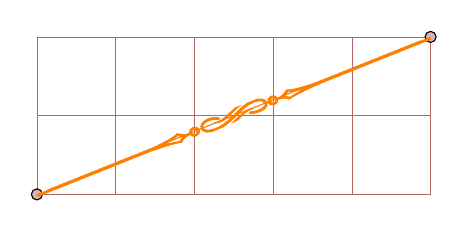
\begin{tikzpicture}
\node (A) at (0,0) {};
\node (B) at (5,2) {};
\draw [help lines,color=Maroon!60]  (0,0) grid (5,2);
\draw [fill=Maroon!30]  (A) circle (2pt) (B) circle (2pt);
\draw [orange] (A)  to [ornament=88]   (B);
\end{tikzpicture}
\end{tkzexample}
\end{minipage}
\begin{minipage}{0.4\textwidth}
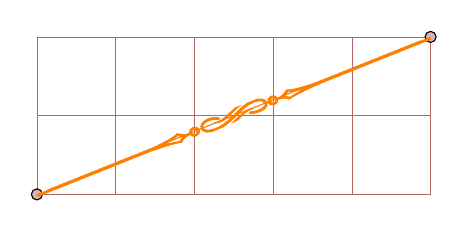
\begin{tikzpicture}
\node (A) at (0,0) {};
\node (B) at (5,2) {};
\draw [help lines,color=Maroon!60]  (0,0) grid (5,2);
\draw [fill=Maroon!30]  (A) circle (2pt) (B) circle (2pt);
\draw [orange] (A)  to [ornament=88]   (B);
\end{tikzpicture}
\end{minipage}
我们还可以用两个装饰来连接两个点\\
\begin{minipage}{0.6\textwidth}
\begin{tkzexample}[code only,small]
	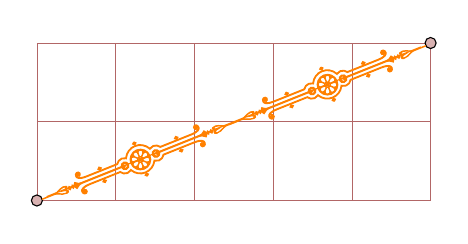
\begin{tikzpicture}
	\node (A) at (0,0) {};
	\node (B) at (5,2) {};
	\draw [help lines,color=Maroon!60]  (0,0) grid (5,2);
	\draw [fill=Maroon!30]  (A) circle (2pt) (B) circle (2pt);
	\path (A)--(B) coordinate[pos=.5] (c1);
	\draw [orange] (A)  to [ornament=84]
	               (c1) to [ornament=84] (B);
	\end{tikzpicture}
\end{tkzexample}
\end{minipage}
\begin{minipage}{0.6\textwidth}
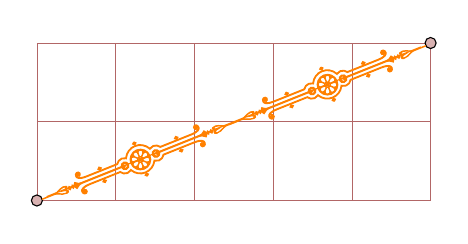
\begin{tikzpicture}
	\node (A) at (0,0) {};
	\node (B) at (5,2) {};
	\draw [help lines,color=Maroon!60]  (0,0) grid (5,2);
	\draw [fill=Maroon!30]  (A) circle (2pt) (B) circle (2pt);
	\path (A)--(B) coordinate[pos=.5] (c1);
	\draw [orange] (A)  to [ornament=84]
	               (c1) to [ornament=84] (B);
	\end{tikzpicture}
\end{minipage}

如果加载了Ti$k$Z的\verb|shapes.geometric|库,我们还可以做出如下花边多边形(实际的多边形边数可以自行选择,比如六边形,然后设置rotate=30)\\
\begin{minipage}{0.6\textwidth}
\begin{tkzexample}[code only,small]
 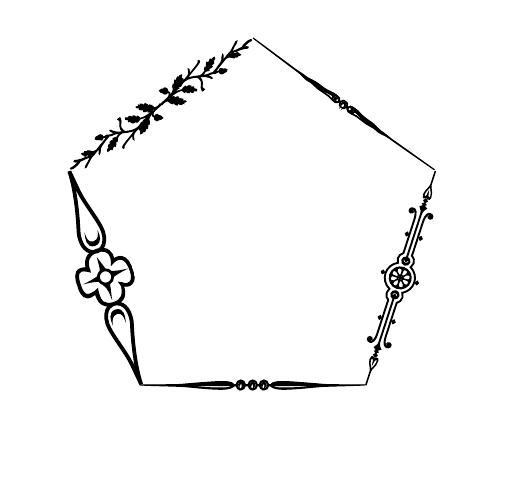
\begin{tikzpicture}[every node={anchor=center,
                                 inner sep=0pt}]
 \node[regular polygon, regular polygon sides=5,
 rotate=36,minimum size=6cm,inner sep=0pt](s)  {};
 \path (s.side 1) to [ornament=81] (s.side 2)
                  to [ornament=83] (s.side 3)
                  to [ornament=84] (s.side 4)
                  to [ornament=86] (s.side 5)
                  to [ornament=87] (s.side 1);
 \end{tikzpicture}
\end{tkzexample}
\end{minipage}
\begin{minipage}{0.4\textwidth}
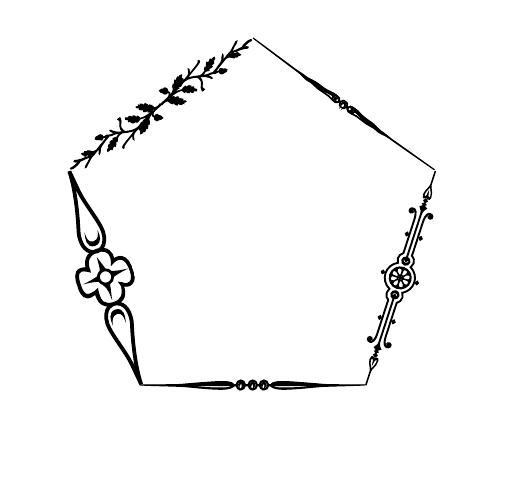
\begin{tikzpicture}[every node={anchor=center,
                                 inner sep=0pt}]
 \node[regular polygon, regular polygon sides=5,
 rotate=36,minimum size=6cm,inner sep=0pt](s)  {};
 \path (s.side 1) to [ornament=81] (s.side 2)
                  to [ornament=83] (s.side 3)
                  to [ornament=84] (s.side 4)
                  to [ornament=86] (s.side 5)
                  to [ornament=87] (s.side 1);
 \end{tikzpicture}
\end{minipage}

最后呢,我们引用源文档中的一个漂亮的装饰环境来结束本文,因为代码略长,我就不在这里引用了,放在此链接中
\href{https://paste.ubuntu.com/p/NpxF2h8q9S/}{https://paste.ubuntu.com/p/NpxF2h8q9S/}。
      \begin{figure}[h!]\centering
        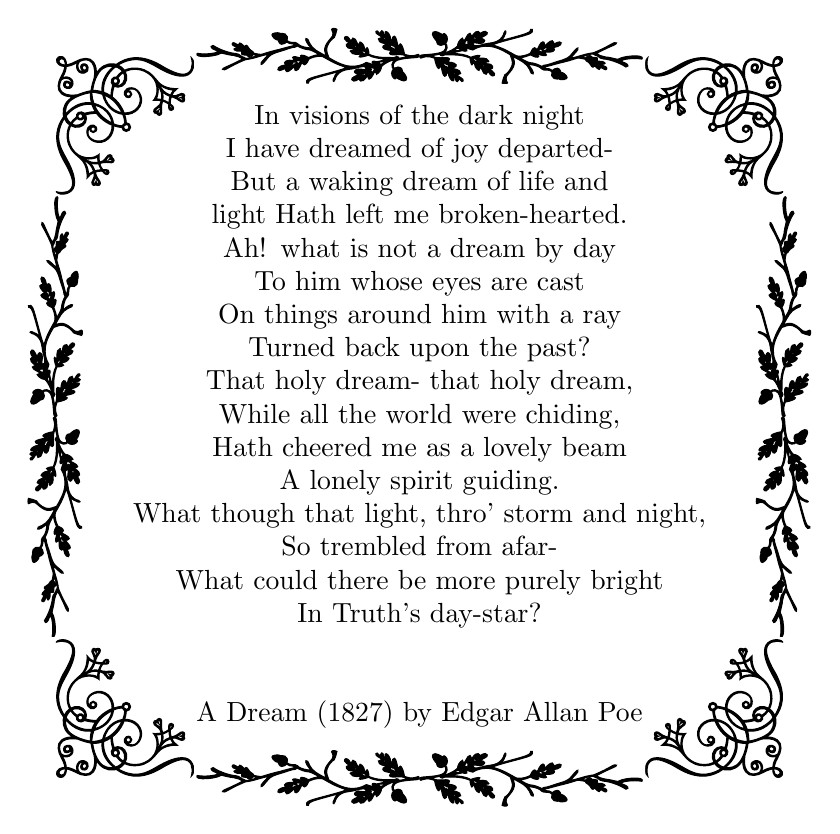
\begin{tikzpicture}
        \node[text width=8cm,align=center](Text){%
        In visions of the dark night\\
        I have dreamed of joy departed-\\
        But a waking dream of life and light\
        Hath left me broken-hearted.\\

        Ah! what is not a dream by day\\
        To him whose eyes are cast \\
        On things around him with a ray \\
        Turned back upon the past? \\

        That holy dream- that holy dream,\\
        While all the world were chiding,\\
        Hath cheered me as a lovely beam\\
        A lonely spirit guiding.\\

        What though that light, thro' storm and night,\\
        So trembled from afar- \\
        What could there be more purely bright \\
        In Truth's day-star? \\
        \vspace{24pt}
         A Dream (1827) by Edgar Allan Poe
        } ;

        \node[inner sep=0pt,shift={(-.5cm,.5cm)},anchor=north west](CNW)  at (Text.north west)
             {\pgfornament[width=1.75cm]{61}};
        \node[inner sep=0pt,shift={(.5cm,.5cm)},anchor=north east](CNE)   at (Text.north east)
             {\pgfornament[width=1.75cm,symmetry=v]{61}};
        \node[inner sep=0pt,shift={(-.5cm,-.5cm)},anchor=south west](CSW) at (Text.south west)
             {\pgfornament[width=1.75cm,symmetry=h]{61}};
        \node[inner sep=0pt,shift={(.5cm,-.5cm)},anchor=south east](CSE)  at (Text.south east)
             {\pgfornament[width=1.75cm,symmetry=c]{61}};
        \pgfornamenthline{CNW}{CNE}{north}{87}
        \pgfornamenthline{CSW}{CSE}{south}{87}
        \pgfornamentvline{CNW}{CSW}{west}{87}
        \pgfornamentvline{CNE}{CSE}{east}{87}
        \end{tikzpicture}
        \caption{A poem}
      \end{figure}






\end{document} 